\section{Задача протекания}

\subsection{Постановка задачи}
Рассмотрим область $\Omega_x = [0,10]$. Для системы (\ref{system:1}) зададим начальные и граничные условия, которые определяются следующим образом:
\begin{equation}
\label{flowout:1}
\begin{aligned}
  & \rho(0, x) = 1, \; x \in [0; 10] \\
  & u(0, x) = 0,    \; x \in [0; 10] \\
  & u(t, 0) = \tilde u, \; t \in [0; T] \\
  & \rho(t, 0) = \tilde \rho, \; t \in [0; T] \\
  & \left.\frac{\partial u}{\partial x}\right|_{x=10} = 0,
   \; t \in [0; T] \\
\end{aligned}
\end{equation}

Где $\tilde v > 0$ и $\tilde \rho \geq 1$. 
Также положим $f$ и $f_0$ из правой части (\ref{system:3}) тождественно равными нулю. \\

Область $\Omega=[0, T] \times[0,10],$ а функции $f$ и $f_{0}$ тождественно равны $0 .$ Параметры $v(v>0)$ и $\tilde{\rho} \tilde{\rho} \geq 1$ задают скорость и плотность, "набегающего" потока.

Вычисления будут проводится до времени $T = N_{0} \tau$, при котором решение перестанет зависеть от времени (выйдет на стационар).
Критерием выхода на стационар будем считать
$$
  \left\| V^{N_{0}} - V_{m}^{N_{0}-50} \right\|_C =
  \max_{m = 0 \dots M} \left| V_{m}^{N_{0}} - V_{m}^{N_{0}-50} \right| 
  \leq \varepsilon
$$
где величина $\varepsilon$ является достаточно малой и определяется опытным путем. \\


\subsection{Разностная схема}
Для решения данной задачи необходимо модифицировать схему. 
Уравнение $V_M^{n+1} = 0$ заменяется на 
$$ V_{M}^{n+1} - V_{M-1}^{n+1} = 0$$

Иные граничные условия при $m=0$:
$$ G_0^{n+1} = \ln(\tilde \rho) $$
$$ V_0^{n+1} = \tilde u $$

Третье уравнение системы (\ref{system:4}) в силу условия (\ref{flowout:1}) заменяется на 
\begin{equation*}
  G_{t,M} + 0.5 [(V \hat G)_{\bar x, M} + V_{M} \hat G_{\bar x, M}] 
      + 0.5h [ (GV)_{x \bar x, M-1} - 0.5  (GV)_{x \bar x, M-2}]  
      + 0.5h [V_M G_{x \bar x, M-1} - 0.5 V_M G_{x \bar x, M-2}] = 0
\end{equation*}
\begin{equation*}
  G_{t,M} + 0.5 [(V \hat G)_{\bar x, M} + V_{M} \hat G_{\bar x, M}]
      + 0.5h [(GV)_{x \bar x, M-1} + V G_{x \bar x, M-1}]  
     - 0.25h [(GV)_{x \bar x, M-2} + V G_{x \bar x, M-2}] = 0
\end{equation*}
\begin{multline*}
  \frac{G_{M}^{n+1} - G_{M}^{n}}{\tau} 
  + \frac12 \left[
      \frac{V_{M}^{n} G_{M}^{n+1} - V_{M-1}^{n} G_{M-1}^{n+1}}{h} 
    + V_{M}^{n} \frac{G_{M}^{n+1} - G_{M-1}^{n+1}}{h}
  \right] +{} \\ {}+
  \frac{h}{2} \left[
      \frac{G_{M-2}^{n} V_{M-2}^{n} - 2 G_{M-1}^{n} V_{M-1}^{n} + G_{M}^{n} V_{M}^{n}}{h^2} +
      V_{M}^{n} \frac{G_{M-2}^{n} - 2 G_{M-1}^{n} + G_{M}^{n}}{h^2}
  \right] -{} \\ {}-
  \frac{h}{4} \left[
      \frac{G_{M-3}^{n} V_{M-3}^{n} - 2 G_{M-2}^{n} V_{M-2}^{n} + G_{M-1}^{n} V_{M-1}^{n}}{h^2} +
      V_{M}^{n} \frac{G_{M-3}^{n} - 2 G_{M-2}^{n} + G_{M-1}^{n}}{h^2}
  \right] = 0
\end{multline*}

\begin{equation*}
  G_{M-1}^{n+1} \left( - \frac{V_{M-1}^{n} + V_{M}^{n}}{2h} \right) +
  G_{M}^{n+1} \left( \frac{1}{\tau} + \frac{V_{M}^{n}}{h} \right) = B_{M}^{n}
\end{equation*}
\begin{multline*}
   B_{M}^{n} =  G_{M}^{n} \left( \frac{1}{\tau} \right)-
  \frac{1}{2h} \left[
    G_{M-2}^{n} V_{M-2}^{n} - 2 G_{M-1}^{n} V_{M-1}^{n} + G_{M}^{n} V_{M}^{n} + 
    V_{M}^{n} (G_{M-2}^{n} - 2 G_{M-1}^{n} + G_{M}^{n})
    \right] +{} \\ {}+
  \frac{1}{4h} \left[
    G_{M-3}^{n} V_{M-3}^{n} - 2 G_{M-2}^{n} V_{M-2}^{n} + G_{M-1}^{n} V_{M-1}^{n} + 
    V_{M}^{n} (G_{M-3}^{n} - 2 G_{M-2}^{n} + G_{M-1}^{n})
    \right]
\end{multline*}


\newpage
\subsection{Численные эксперименты}
Рассматривается задача (\ref{flowout:1}).
Зафиксируем $$ \tau = 10^{-3}, \; h = 10^{-2}, \; \varepsilon = 10^{-2}$$

Будем рассматривать зависимости 
$ p(\rho) = C \rho $ и $p(\rho) = \rho^{\gamma}$
и внешние параметры 
$$ (C, \mu) \in \{1, 10, 100\} \times \{0.1, 0.01, 0.001\}, \; \gamma = 1.4$$

\subsubsection{Стабилизация решения}
Далее приведены таблицы зависимости времени стабилизации $N_0 \tau$ 
от параметров $\mu$, $C$, $\tilde \rho$ и $\tilde u$.
\begin{table}[H]
\centering
\begin{tabular}{|c|c|c|c|c|}
\hline
\diagPU & \texttt{1} & \texttt{2} & \texttt{3} & \texttt{4} \\ \hline
 \texttt{1} & \texttt{7.730} & \texttt{26.261} & \texttt{10.136} & \texttt{6.274} \\ \hline
 \texttt{2} & \texttt{6.686} & \texttt{15.668} & \texttt{7.586}  & \texttt{4.951} \\ \hline
 \texttt{3} & \texttt{6.101} & \texttt{12.863} & \texttt{6.659}  & \texttt{4.442} \\ \hline
 \texttt{4} & \texttt{5.723} & \texttt{11.453} & \texttt{6.153}  & \texttt{4.159} \\ \hline
\end{tabular}
\caption{Время стабилизации при $C = 1$, $\gamma = 1$ и~$\mu = 0.1$.}
\end{table}

\begin{table}[H]
\centering
\begin{tabular}{|c|c|c|c|c|}
\hline
\diagPU & \texttt{1} & \texttt{2} & \texttt{3} & \texttt{4} \\ \hline
 \texttt{1} & \texttt{7.067} & \texttt{7.897} & \texttt{7.183} & \texttt{5.489}  \\ \hline
 \texttt{2} & \texttt{7.905} & \texttt{5.503} & \texttt{3.038} & \texttt{26.221} \\ \hline
 \texttt{3} & \texttt{7.158} & \texttt{3.043} & \texttt{2.359} & \texttt{5.817}  \\ \hline
 \texttt{4} & \texttt{5.419} & \texttt{2.415} & \texttt{2.132} & \texttt{3.888}  \\ \hline
\end{tabular}
\caption{Время стабилизации при $C = 10$, $\gamma = 1$ и~$\mu = 0.1$.}
\end{table}

\begin{table}[H]
\centering
\begin{tabular}{|c|c|c|c|c|}
\hline
\diagPU & \texttt{1} & \texttt{2} & \texttt{3} & \texttt{4} \\ \hline
 \texttt{1} & \texttt{8.184} & \texttt{8.346} & \texttt{6.619} & \texttt{5.821} \\ \hline
 \texttt{2} & \texttt{7.454} & \texttt{5.799} & \texttt{5.561} & \texttt{4.606} \\ \hline
 \texttt{3} & \texttt{5.604} & \texttt{4.238} & \texttt{4.877} & \texttt{6.615} \\ \hline
 \texttt{4} & \texttt{5.348} & \texttt{4.749} & \texttt{6.964} & \texttt{7.566} \\ \hline
\end{tabular}
\caption{Время стабилизации при $C = 100$, $\gamma = 1$ и~$\mu = 0.1$.}
\end{table}

\begin{table}[H]
\centering
\begin{tabular}{|c|c|c|c|c|}
\hline
\diagPU & \texttt{1} & \texttt{2} & \texttt{3} & \texttt{4} \\ \hline
 \texttt{1} & \texttt{6.905} & \texttt{55.486} & \texttt{14.283} & \texttt{7.916} \\ \hline
 \texttt{2} & \texttt{5.764} & \texttt{32.822} & \texttt{10.457} & \texttt{6.256} \\ \hline
 \texttt{3} & \texttt{5.195} & \texttt{4.295}  & \texttt{9.147}  & \texttt{5.623} \\ \hline
 \texttt{4} & \texttt{4.864} & \texttt{3.961}  & \texttt{8.456}  & \texttt{5.274} \\ \hline
\end{tabular}
\caption{Время стабилизации при $C = 1$, $\gamma = 1.4$ и~$\mu = 0.1$.}
\end{table}

\begin{table}[H]
\centering
\begin{tabular}{|c|c|c|c|c|}
\hline
\diagPU & \texttt{1} & \texttt{2} & \texttt{3} & \texttt{4} \\ \hline
 \texttt{1} & \texttt{8.601} & \texttt{25.736} & \texttt{9.438} & \texttt{5.662} \\ \hline
 \texttt{2} & \texttt{6.875} & \texttt{15.399} & \texttt{7.302} & \texttt{4.667} \\ \hline
 \texttt{3} & \texttt{6.286} & \texttt{12.688} & \texttt{6.511} & \texttt{4.351} \\ \hline
 \texttt{4} & \texttt{6.037} & \texttt{11.344} & \texttt{6.051} & \texttt{4.239} \\ \hline
\end{tabular}
\caption{Время стабилизации при $C = 1$, $\gamma = 1$ и~$\mu = 0.01$.}
\end{table}

\begin{table}[H]
\centering
\begin{tabular}{|c|c|c|c|c|}
\hline
\diagPU & \texttt{1} & \texttt{2} & \texttt{3} & \texttt{4} \\ \hline
 \texttt{1} & \texttt{10.469} & \texttt{9.959}   & \texttt{8.658} & \texttt{6.810}  \\ \hline
 \texttt{2} & \texttt{9.776}  & \texttt{6.741}   & \texttt{3.988} & \texttt{26.934} \\ \hline
 \texttt{3} & \texttt{8.230}  & \texttt{3.957}   & \texttt{2.365} & \texttt{13.669} \\ \hline
 \texttt{4} & \texttt{6.083}  & \texttt{138.938} & \texttt{2.276} & \texttt{4.899}  \\ \hline
\end{tabular}
\caption{Время стабилизации при $C = 10$, $\gamma = 1$ и~$\mu = 0.01$.}
\end{table}

\begin{table}[H]
\centering
\begin{tabular}{|c|c|c|c|c|}
\hline
\diagPU & \texttt{1} & \texttt{2} & \texttt{3} & \texttt{4} \\ \hline
 \texttt{1} & \texttt{8.297}  & \texttt{8.564}  & \texttt{7.710}  & \texttt{5.874}  \\ \hline
 \texttt{2} & \texttt{7.360}  & \texttt{5.692}  & \texttt{6.031}  & \texttt{4.483}  \\ \hline
 \texttt{3} & \texttt{5.470}  & \texttt{4.512}  & \texttt{35.671} & \texttt{19.222} \\ \hline
 \texttt{4} & \texttt{18.271} & \texttt{13.940} & \texttt{12.548} & \texttt{12.381} \\ \hline
\end{tabular}
\caption{Время стабилизации при $C = 100$, $\gamma = 1$ и~$\mu = 0.01$.}
\end{table}

\begin{table}[H]
\centering
\begin{tabular}{|c|c|c|c|c|}
\hline
\diagPU & \texttt{1} & \texttt{2} & \texttt{3} & \texttt{4} \\ \hline
 \texttt{1} & \texttt{8.225} & \texttt{56.153} & \texttt{13.956} & \texttt{7.561} \\ \hline
 \texttt{2} & \texttt{6.426} & \texttt{33.884} & \texttt{10.583} & \texttt{6.296} \\ \hline
 \texttt{3} & \texttt{5.375} & \texttt{25.812} & \texttt{9.397}  & \texttt{5.778} \\ \hline
 \texttt{4} & \texttt{4.992} & \texttt{4.293}  & \texttt{8.730}  & \texttt{5.469} \\ \hline
\end{tabular}
\caption{Время стабилизации при $C = 1$, $\gamma = 1.4$ и~$\mu = 0.01$.}
\end{table}

\begin{table}[H]
\centering
\begin{tabular}{|c|c|c|c|c|}
\hline
\diagPU & \texttt{1} & \texttt{2} & \texttt{3} & \texttt{4} \\ \hline
 \texttt{1} & \texttt{9.509} & \texttt{23.464} & \texttt{8.956} & \texttt{5.536} \\ \hline
 \texttt{2} & \texttt{7.285} & \texttt{15.754} & \texttt{7.361} & \texttt{5.168} \\ \hline
 \texttt{3} & \texttt{6.824} & \texttt{13.275} & \texttt{6.636} & \texttt{5.024} \\ \hline
 \texttt{4} & \texttt{6.553} & \texttt{11.871} & \texttt{6.240} & \texttt{4.958} \\ \hline
\end{tabular}
\caption{Время стабилизации при $C = 1$, $\gamma = 1$ и~$\mu = 0.001$.}
\end{table}

\begin{table}[H]
\centering
\begin{tabular}{|c|c|c|c|c|}
\hline
\diagPU & \texttt{1} & \texttt{2} & \texttt{3} & \texttt{4} \\ \hline
 \texttt{1} & \texttt{10.637} & \texttt{10.405} & \texttt{10.661} & \texttt{7.382}  \\ \hline
 \texttt{2} & \texttt{11.011} & \texttt{7.058}  & \texttt{4.328}  & \texttt{28.522} \\ \hline
 \texttt{3} & \texttt{42.476} & \texttt{51.377} & \texttt{2.436}  & \texttt{24.065} \\ \hline
 \texttt{4} & \texttt{25.933} & \texttt{29.906} & \texttt{2.579}  & \texttt{52.223} \\ \hline
\end{tabular}
\caption{Время стабилизации при $C = 10$, $\gamma = 1$ и~$\mu = 0.001$.}
\end{table}



\begin{table}[H]
\centering
\begin{tabular}{|c|c|c|c|c|}
\hline
\diagPU & \texttt{1} & \texttt{2} & \texttt{3} & \texttt{4} \\ \hline
 \texttt{1} & \texttt{9.066}  & \texttt{49.744} & \texttt{13.503} & \texttt{7.404} \\ \hline
 \texttt{2} & \texttt{7.089}  & \texttt{36.143} & \texttt{11.174} & \texttt{6.488} \\ \hline
 \texttt{3} & \texttt{5.901}  & \texttt{28.363} & \texttt{10.123} & \texttt{6.065} \\ \hline
 \texttt{4} & \texttt{108.792} & \texttt{4.770} & \texttt{9.324}  & \texttt{5.808} \\ \hline
\end{tabular}
\caption{Время стабилизации при $C = 1$, $\gamma = 1.4$ и~$\mu = 0.001$.}
\end{table}


\subsubsection{Динамика процесса}
Рассмотрим случай $C = 1$, $\gamma = 1$, $\mu = 0.1$, $\varepsilon = 10^{-2}$, $\tilde \rho = 1$, $\tilde u = 1$.
Далее приведены срезы графиков $V$ и $G$ (динамика процесса) в разные моменты времени.
\begin{figure}[H]
\center{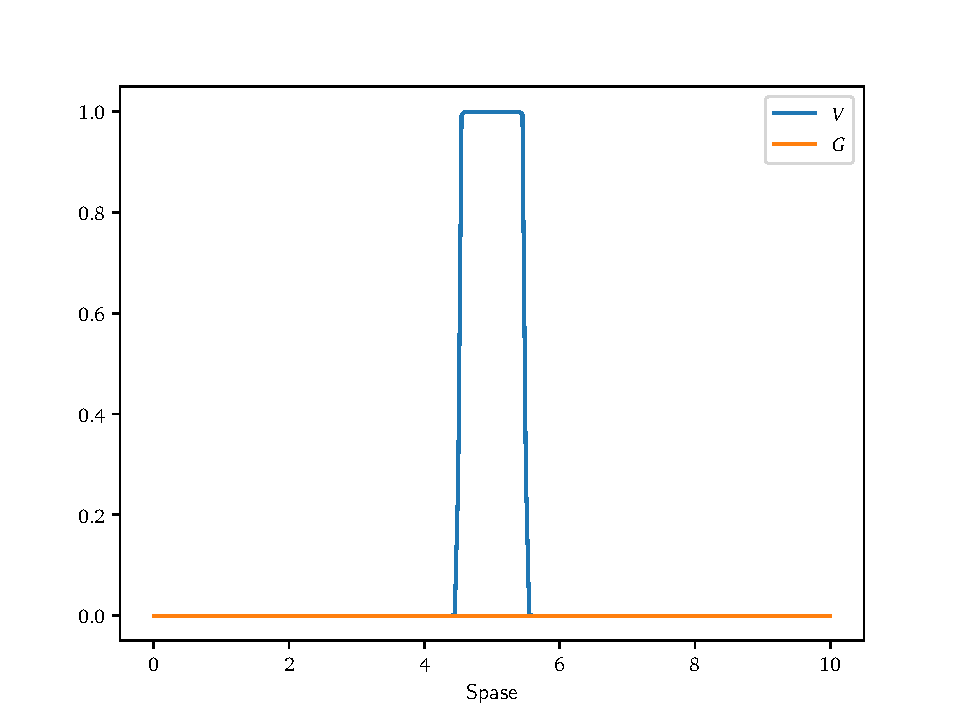
\includegraphics[scale=0.85]{pics_1d_cut/cut_4_1_1_0.1_0.pdf}}
\caption{Срез для $t=0$.}
\end{figure}

\begin{figure}[H]
\center{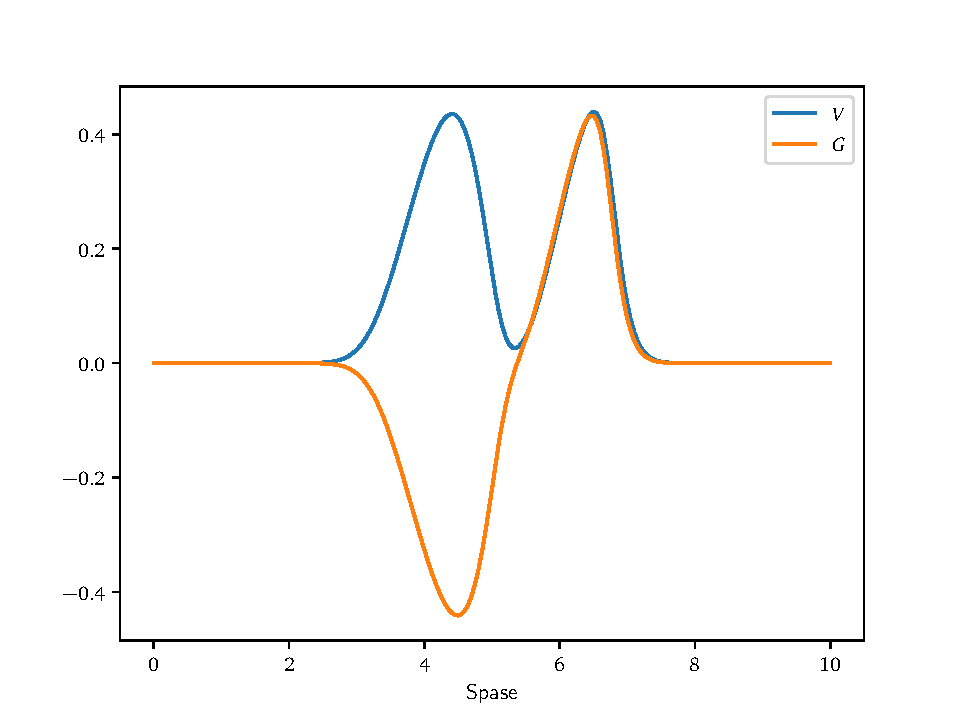
\includegraphics[scale=0.85]{pics_1d_cut/cut_4_1_1_0.1_1.pdf}}
\caption{Срез для $t=1$.}
\end{figure}

\begin{figure}[H]
\center{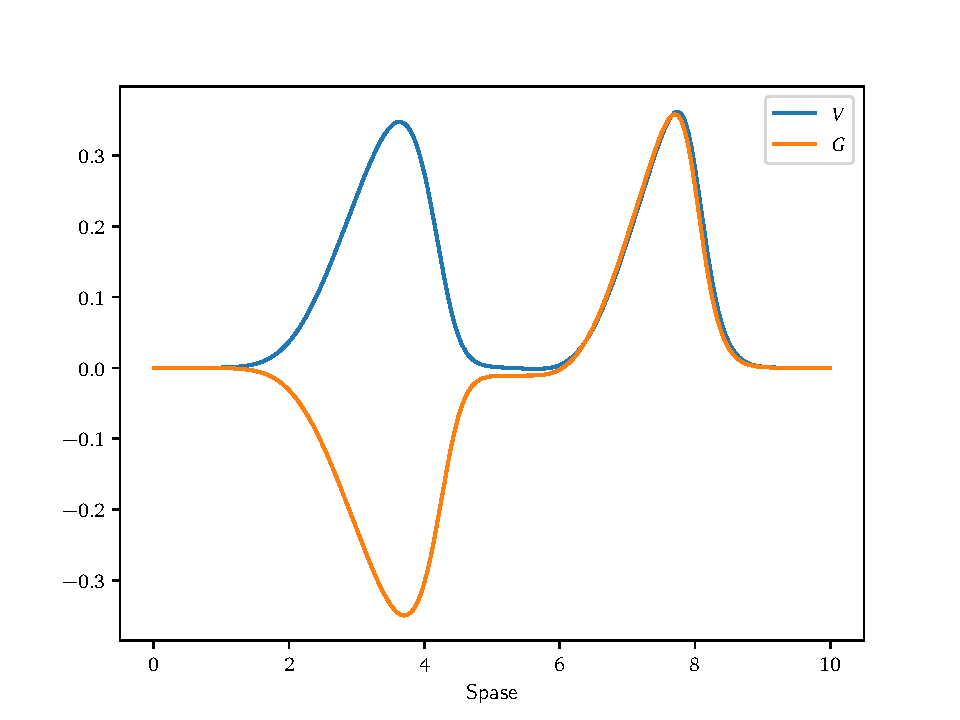
\includegraphics[scale=0.9]{pics_1d_cut/cut_4_1_1_0.1_2.pdf}}
\caption{Срез для $t=2$.}
\end{figure}

\begin{figure}[H]
\center{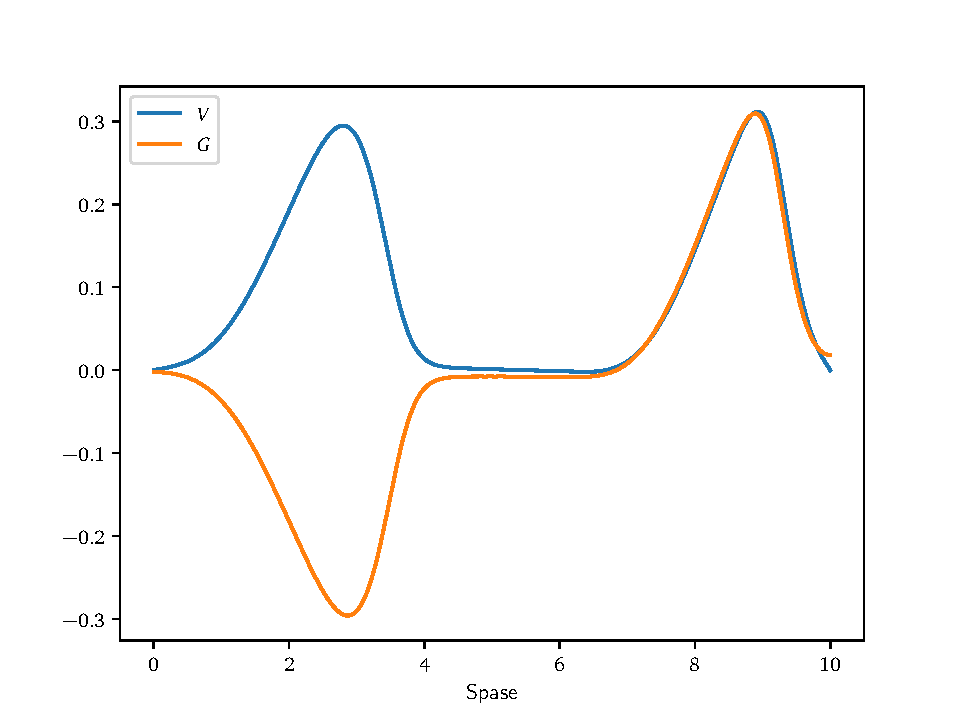
\includegraphics[scale=0.9]{pics_1d_cut/cut_4_1_1_0.1_3.pdf}}
\caption{Срез для $t=3$.}
\end{figure}

\begin{figure}[H]
\center{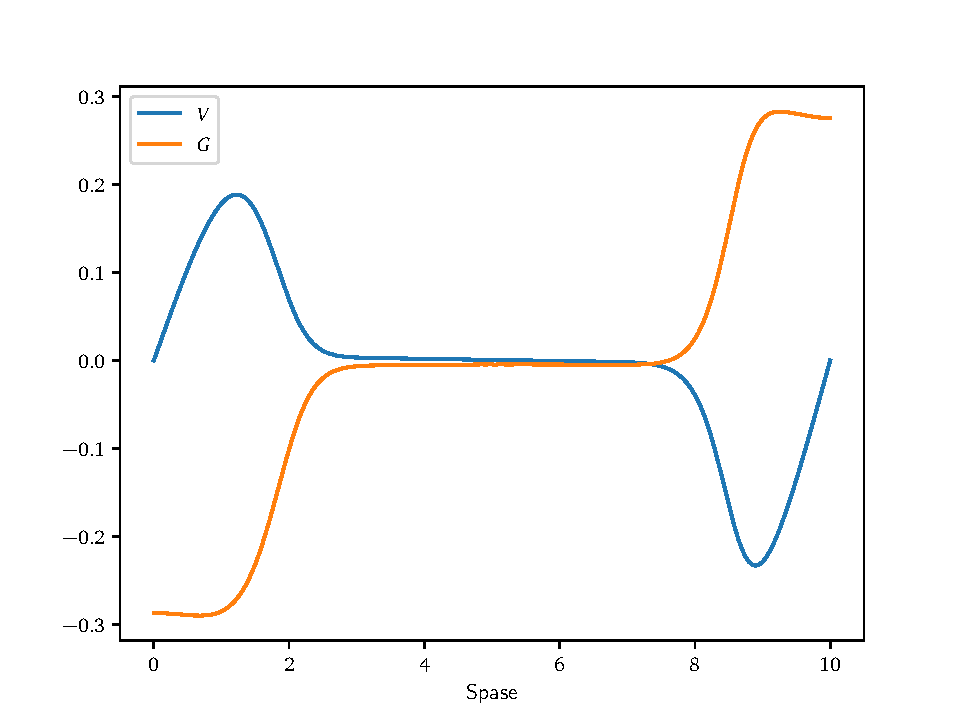
\includegraphics[scale=0.9]{pics_1d_cut/cut_4_1_1_0.1_4.pdf}}
\caption{Срез для $t=5$.}
\end{figure}

\begin{figure}[H]
\center{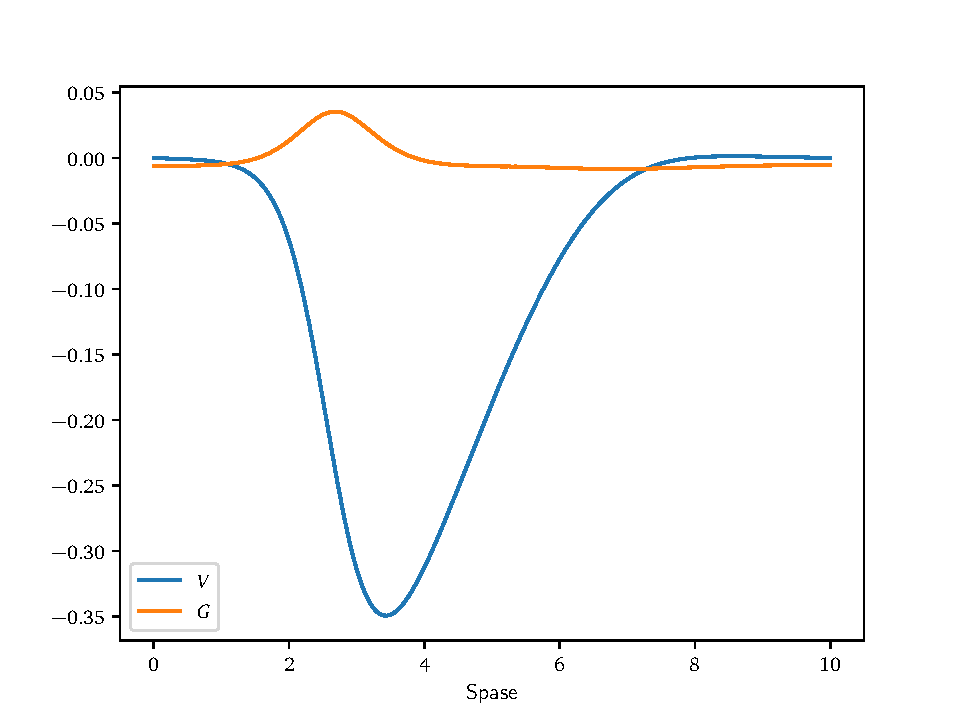
\includegraphics[scale=0.9]{pics_1d_cut/cut_4_1_1_0.1_5.pdf}}
\caption{Срез для $t=10$.}
\end{figure}

\begin{figure}[H]
\center{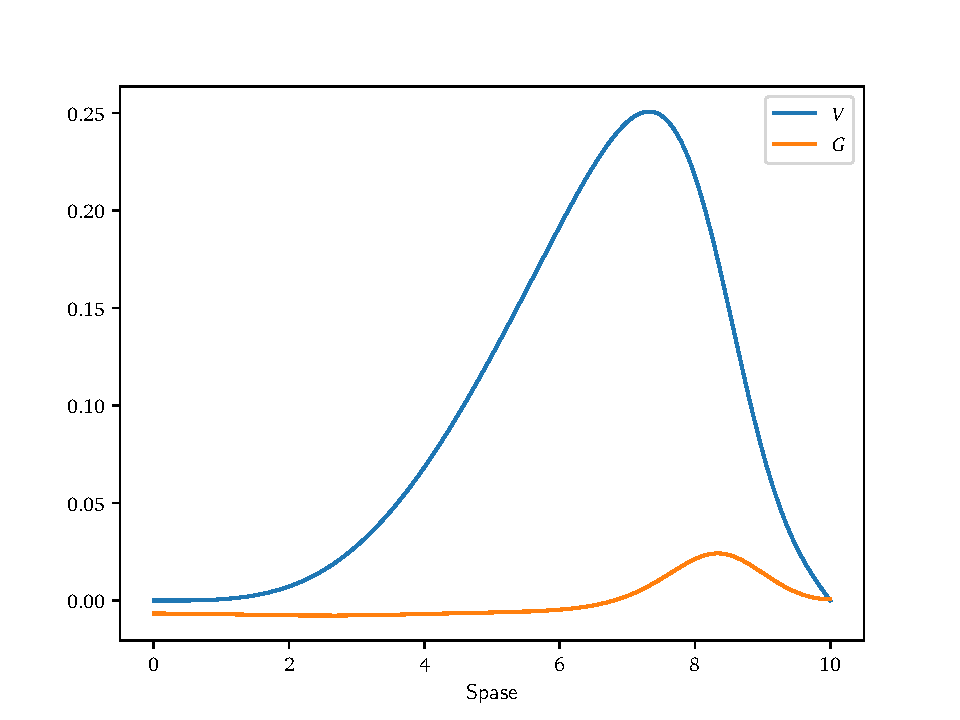
\includegraphics[scale=0.9]{pics_1d_cut/cut_4_1_1_0.1_6.pdf}}
\caption{Срез для $t=20$.}
\end{figure}

\begin{figure}[H]
\center{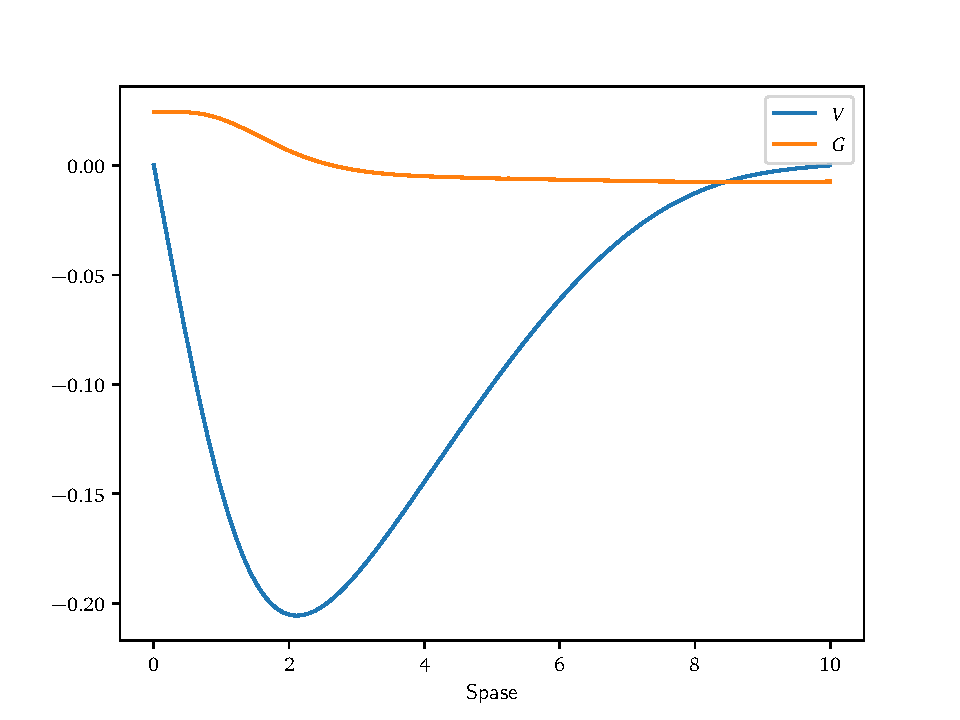
\includegraphics[scale=0.9]{pics_1d_cut/cut_4_1_1_0.1_7.pdf}}
\caption{Срез для $t=30$.}
\end{figure}

\begin{figure}[H]
\center{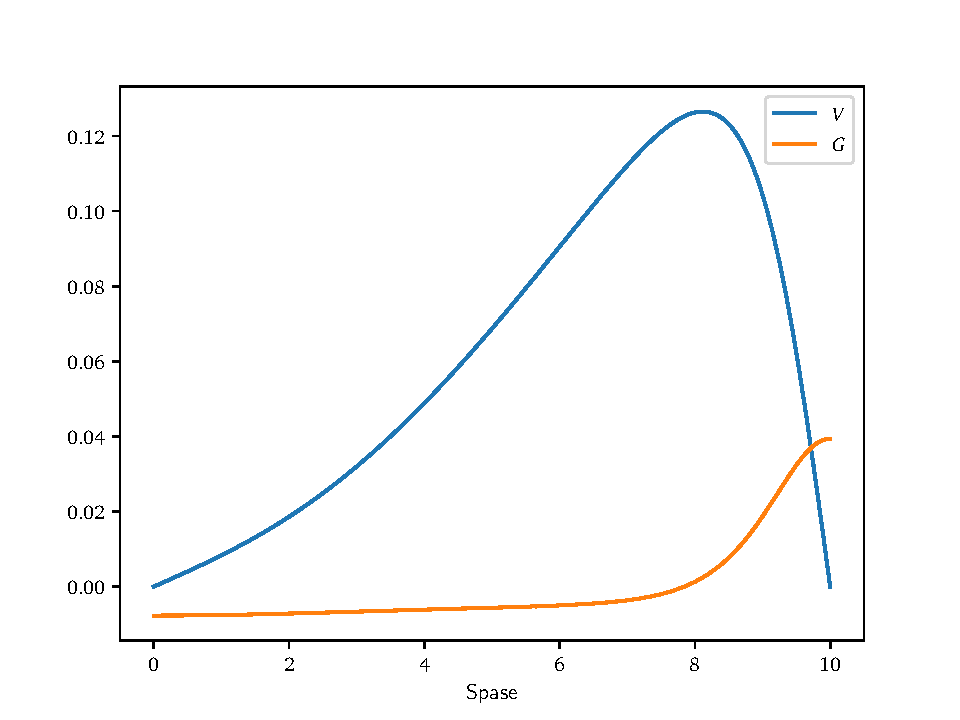
\includegraphics[scale=0.9]{pics_1d_cut/cut_4_1_1_0.1_8.pdf}}
\caption{Срез для $t=60$.}
\end{figure}

\begin{figure}[H]
\center{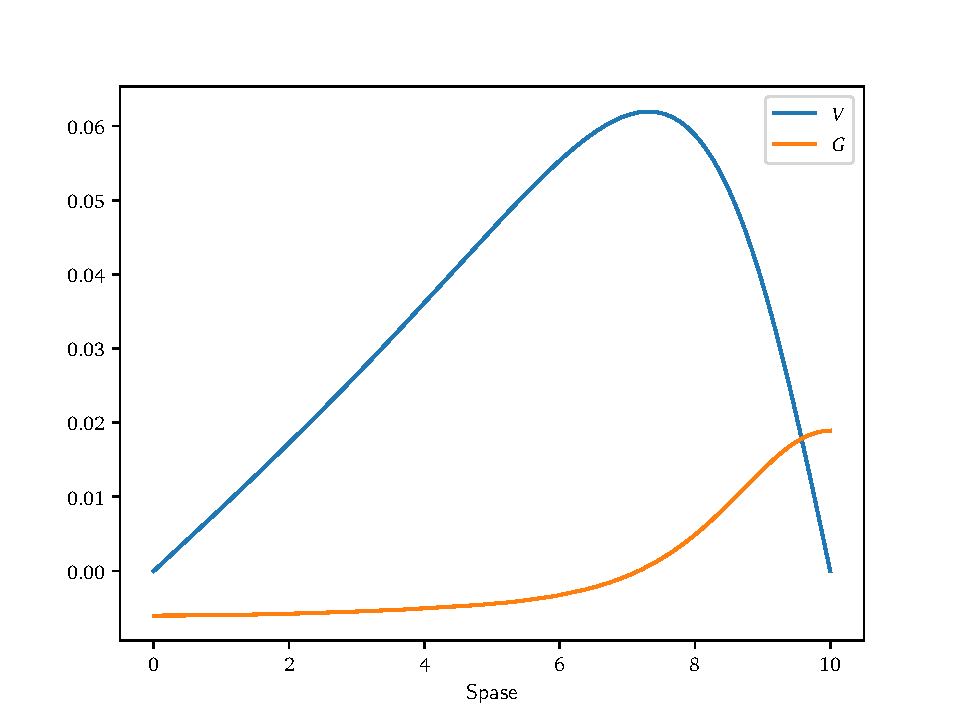
\includegraphics[scale=0.9]{pics_1d_cut/cut_4_1_1_0.1_9.pdf}}
\caption{Срез для $t=120$.}
\end{figure}

\begin{figure}[H]
\center{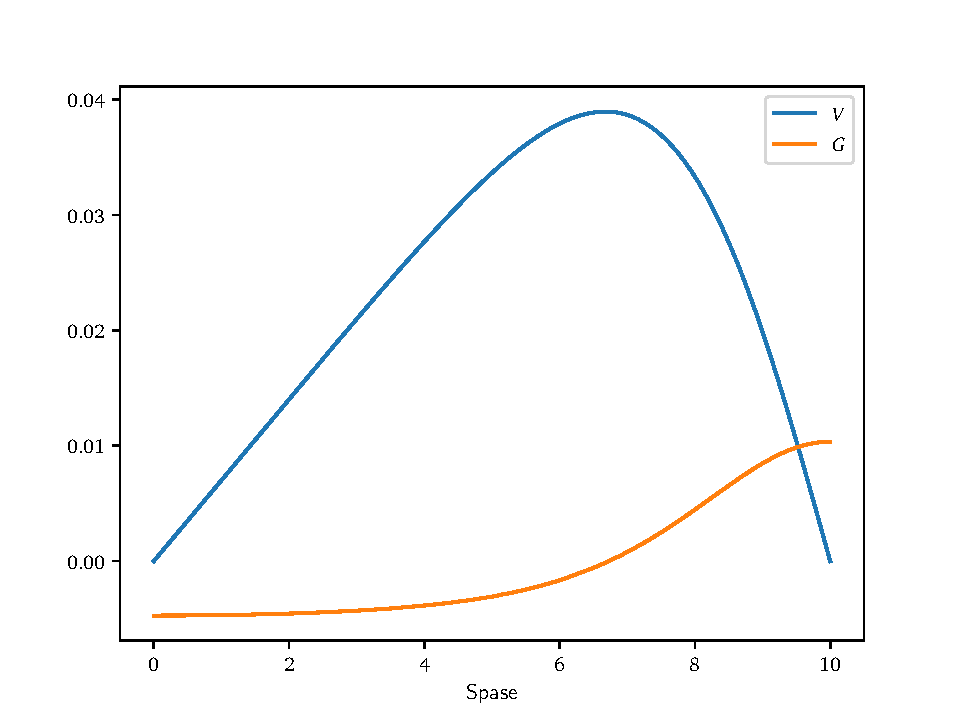
\includegraphics[scale=0.9]{pics_1d_cut/cut_4_1_1_0.1_10.pdf}}
\caption{Срез для $t=180$.}
\end{figure}

\begin{figure}[H]
\center{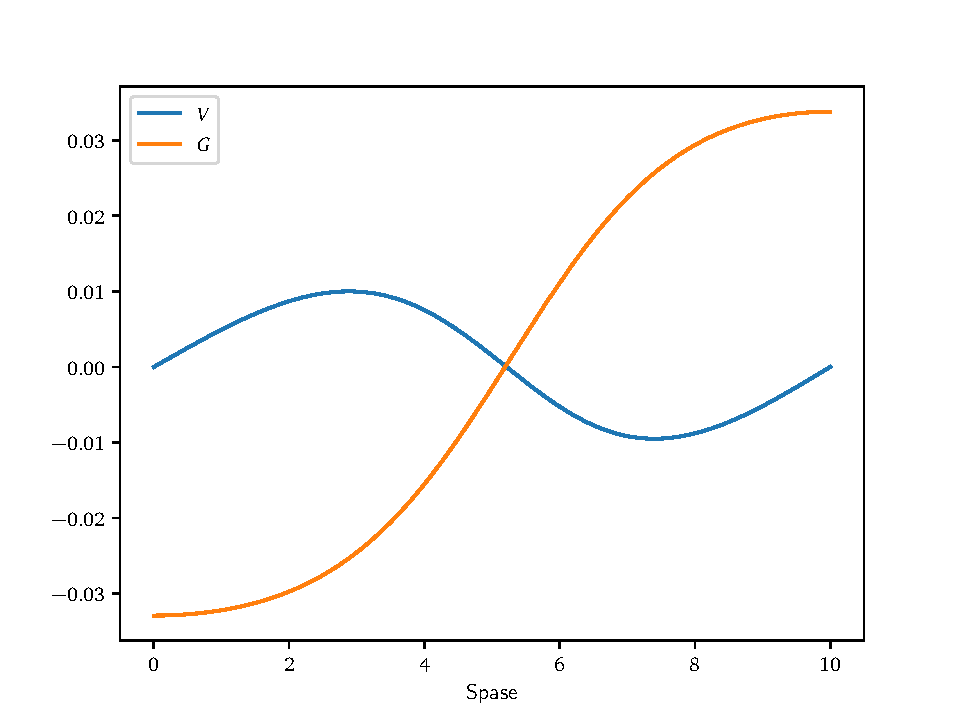
\includegraphics[scale=0.9]{pics_1d_cut/cut_4_1_1_0.1_11.pdf}}
\caption{Срез для $t=184.35$.}
\end{figure}


\subsection{Вывод}
C уменьшением параметра $\mu$ время стабилизации увеличивается. 
Не замечено зависимости времени стабилизации от параметра $C$.
Общей зависимости от пары параметров $(\tilde \rho, \tilde u)$ замечено не было.
